\documentclass[../en-fa-lab.tex]{subfiles}

\usepackage{hyperref}
\hypersetup{
    pdftitle={(EN) L0 - Intro session},   % The title shown in the browser tab
    pdfauthor={},         % Your name or organization
    pdfsubject={},   % A brief description
    pdfkeywords={}
}


\begin{document}

\section{\texorpdfstring{\textbf{Intro session}}{Intro session}}\label{intro-session}

To begin with, make sure you have read the Laboratory Guide on
Moodle. In this lab, you will learn how to write a C/C++ program in
Microsoft Visual Studio or JetBrains CLion. You will also learn how to
generate data for evaluating algorithms and how to create graphs in
Microsoft Office
Excel.

\subsection{Microsoft Visual Studio}\label{microsoft-visual-studio}

\subsubsection{Install}\label{install}

Free edition: \url{https://visualstudio.microsoft.com/vs/community/}

During installation the following package must be chosen:

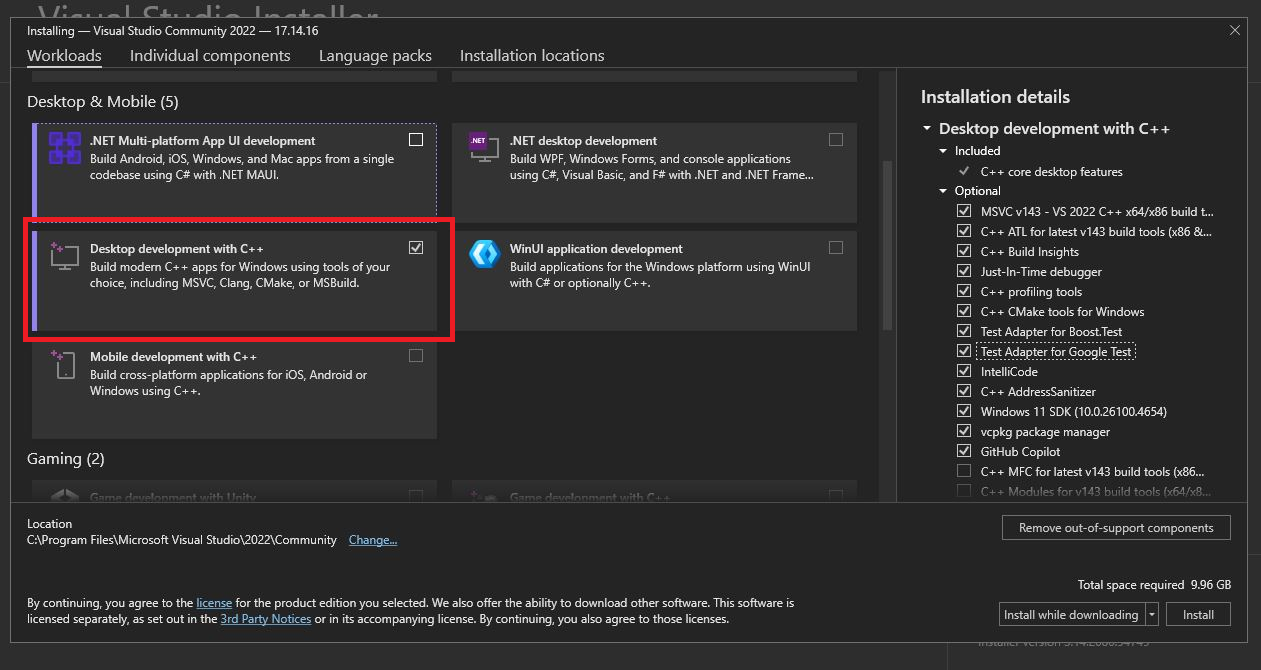
\includegraphics[width=\textwidth]{../Resources/lab0/vs_components.png}

\subsubsection{Use}\label{use}

\begin{enumerate}
\def\labelenumi{\arabic{enumi}.}
\item
    Create project:
%  Create project: \emph{File -\textgreater{} New -\textgreater{} Project\ldots{}}
%\item
%  Project type: \emph{Templates -\textgreater{} Other Languages -\textgreater{} Visual C++ -\textgreater{} Win32 -\textgreater{} Win32 Console App}
\end{enumerate}

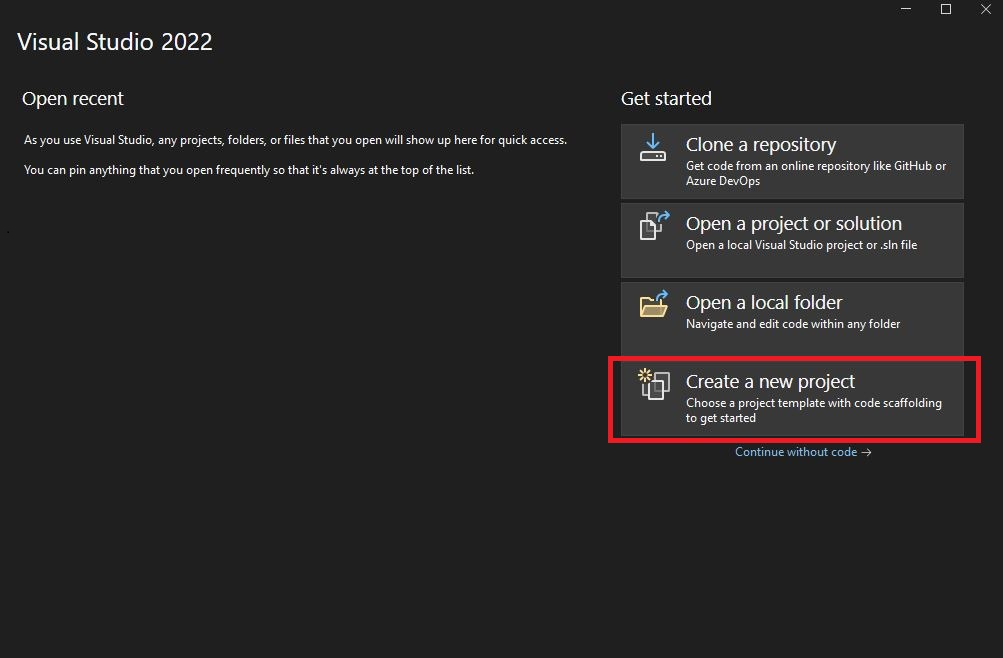
\includegraphics[width=\textwidth]{../Resources/lab0/create_project1.png}
%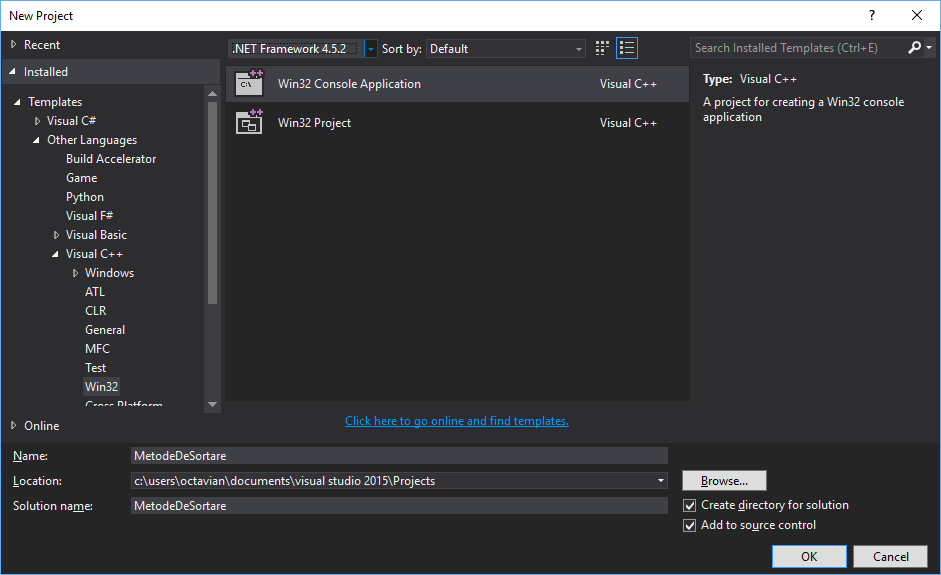
\includegraphics[width=\textwidth]{../Resources/lab0/image1.png}

\begin{enumerate}
\def\labelenumi{\arabic{enumi}.}
\setcounter{enumi}{1}
\item
    Select ``\emph{Empty project}''
%  Project properties: choose ``\emph{Console application}'' and select ``\emph{Empty project}''
\end{enumerate}

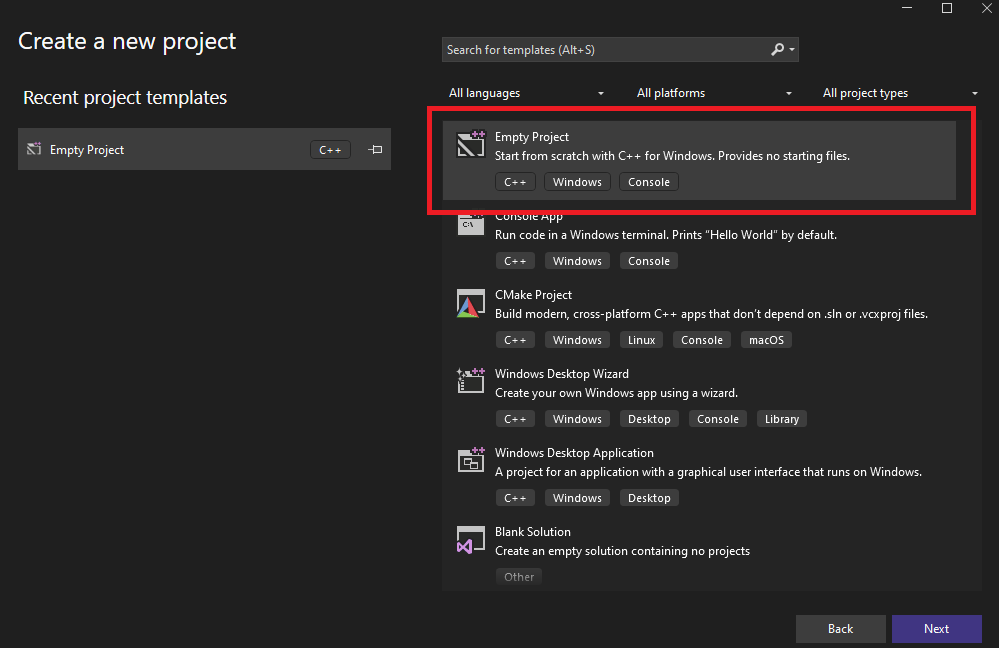
\includegraphics[width=\textwidth]{../Resources/lab0/create_project2.png}
%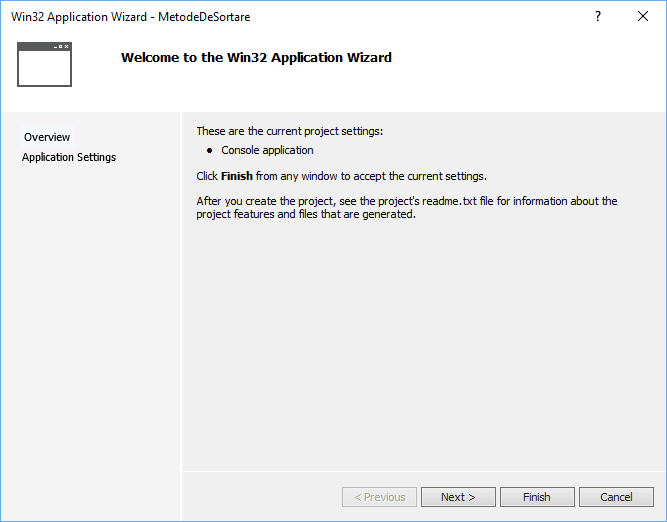
\includegraphics[width=\textwidth]{../Resources/lab0/image2.png}
%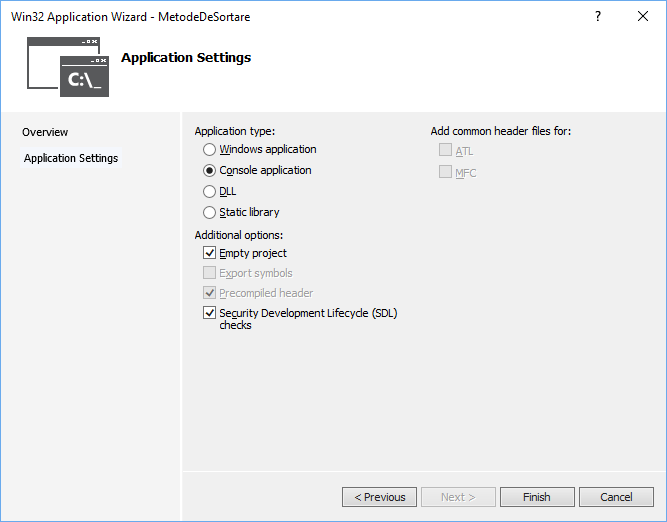
\includegraphics[width=\textwidth]{../Resources/lab0/image3.png}

\begin{enumerate}
\def\labelenumi{\arabic{enumi}.}
\setcounter{enumi}{2}
\item
      Give the project a name.
%Proprietăți proiect: alege ``\emph{Console application}" și bifează ``\emph{Empty project}"
\end{enumerate}

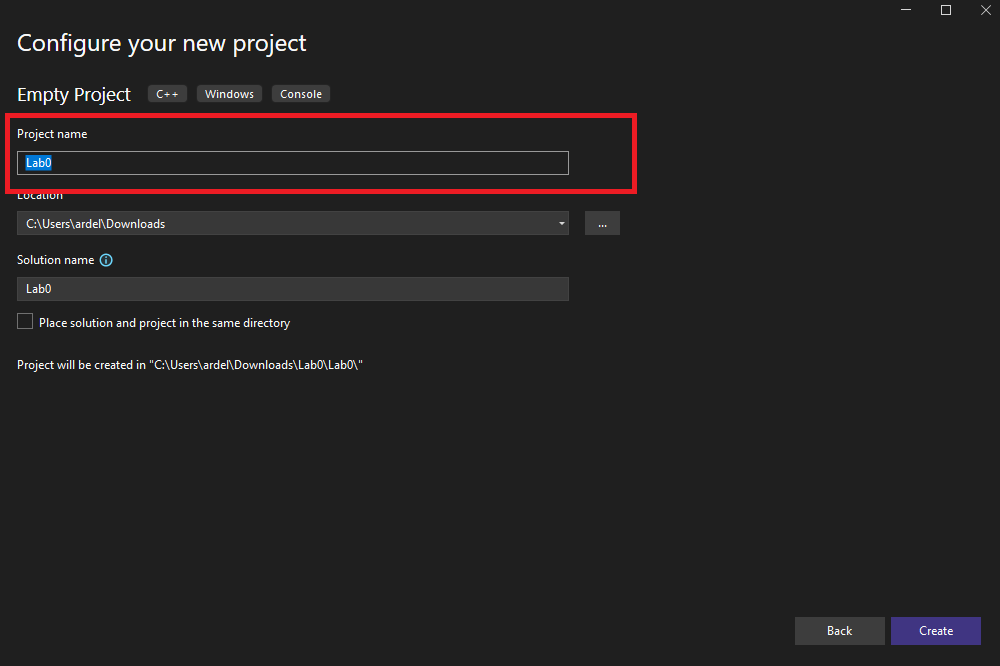
\includegraphics[width=\textwidth]{../Resources/lab0/create_project3.png}

\begin{enumerate}
\def\labelenumi{\arabic{enumi}.}
\setcounter{enumi}{3}
\item
  Create a \emph{*.cpp} file [select from 'Solution Explorer' menu - might be left/right].
\end{enumerate}

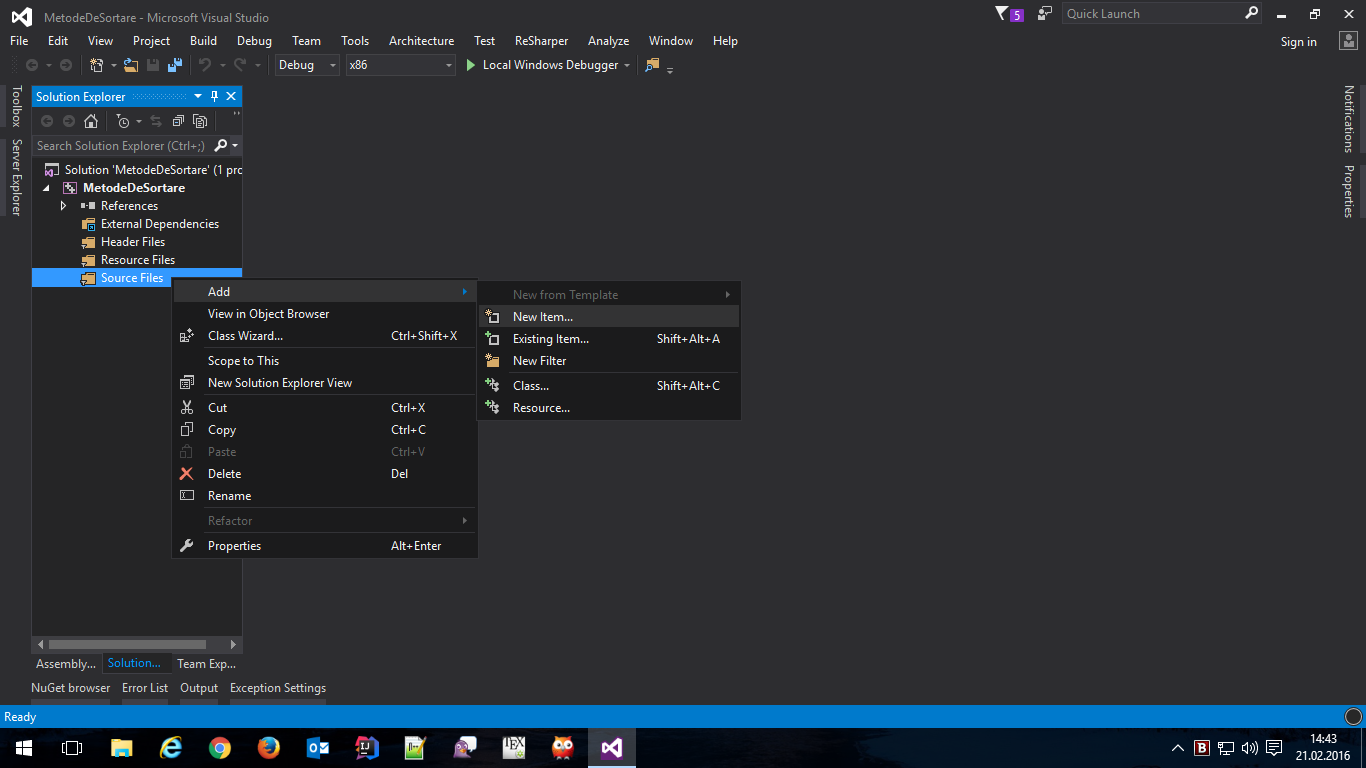
\includegraphics[width=\textwidth]{../Resources/lab0/image4.png}

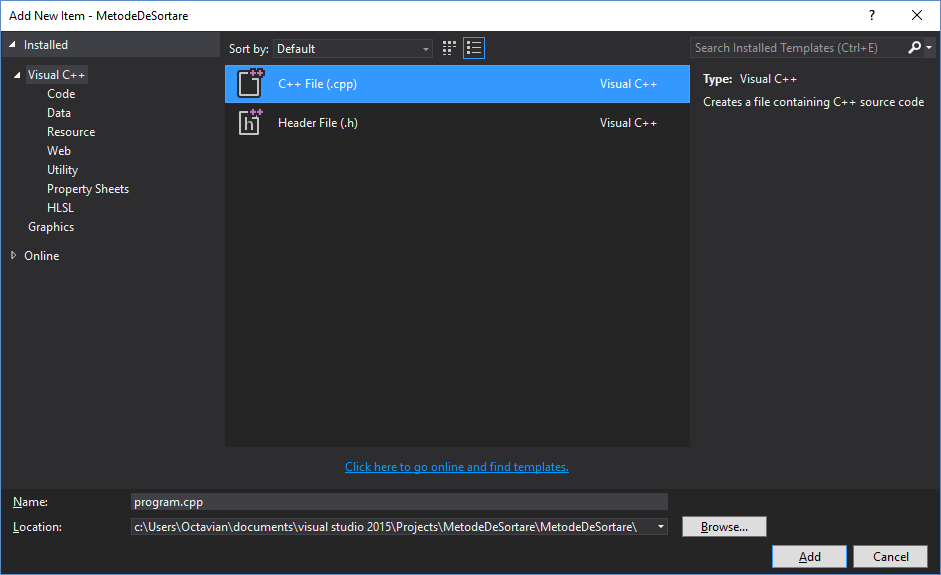
\includegraphics[width=\textwidth]{../Resources/lab0/image5.png}

\begin{enumerate}
\def\labelenumi{\arabic{enumi}.}
\setcounter{enumi}{4}
\item
  Compile and execute the program (in \textbf{DEBUG} mode)
\end{enumerate}

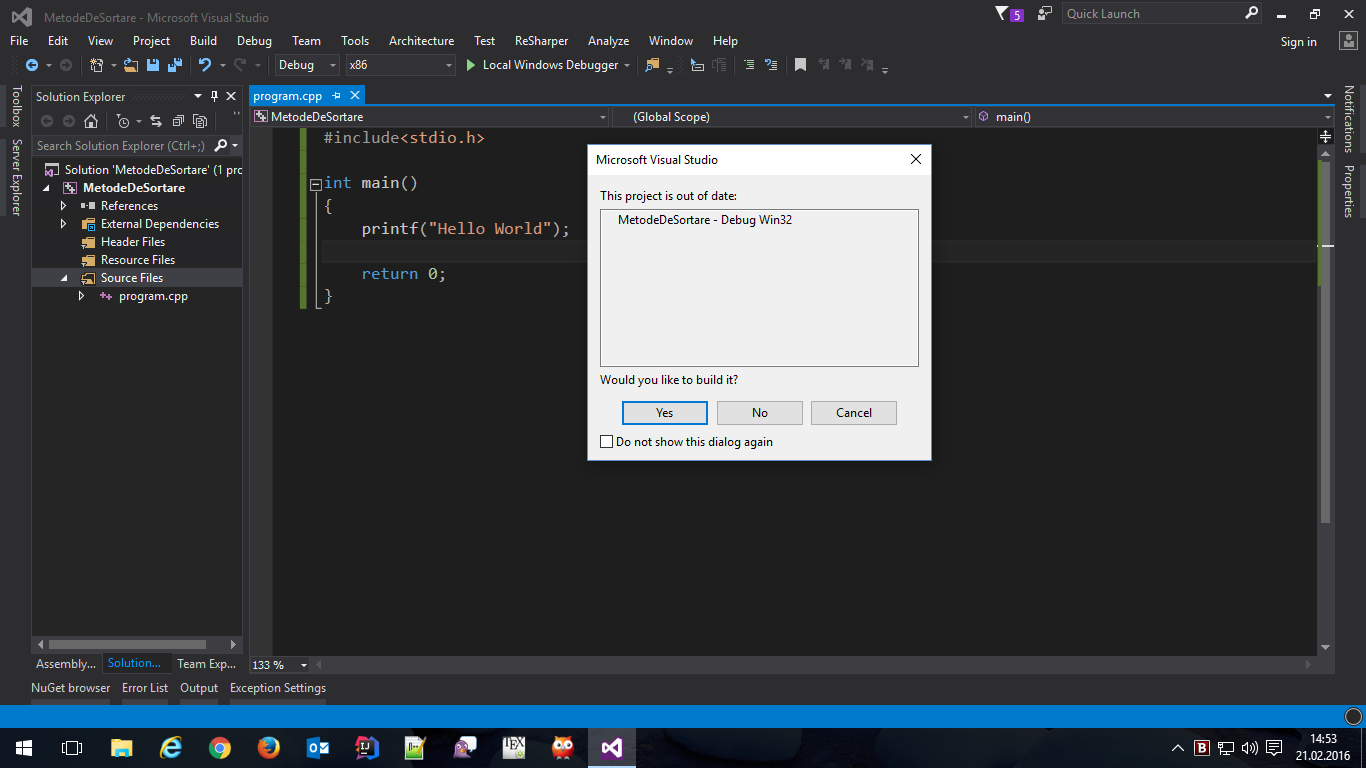
\includegraphics[width=\textwidth]{../Resources/lab0/image6.png}

\subsection{JetBrains CLion}\label{jetbrains-clion}

\subsubsection{Install}\label{install-1}

Register with your student e-mail address: \emph{@student.utcluj.ro} on
https://www.jetbrains.com/student/

Download and install MinGW: https://sourceforge.net/projects/mingw/

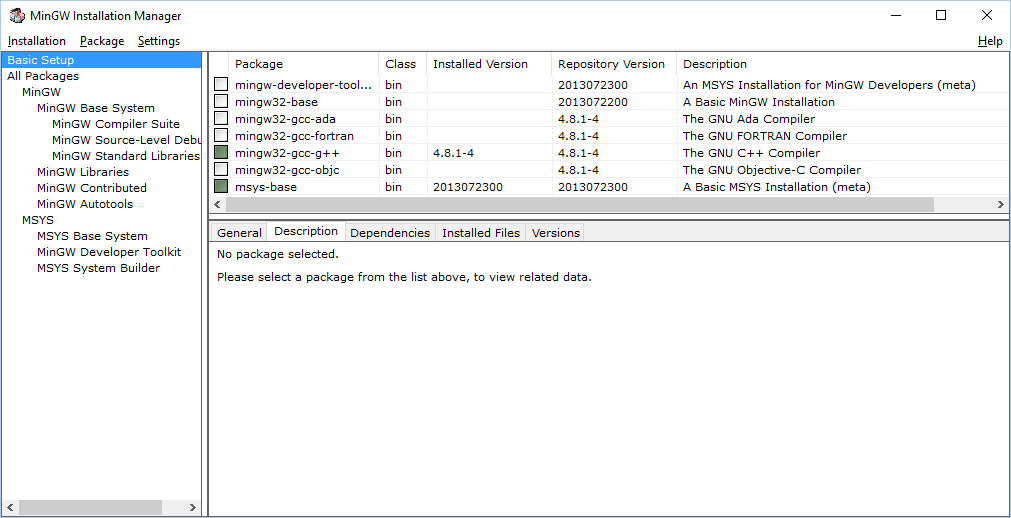
\includegraphics[width=\textwidth]{../Resources/lab0/image7.png}

Download and install CLion:
\url{https://www.jetbrains.com/clion/download/\#section=windows}

\subsubsection{Use}\label{use-1}

\begin{enumerate}
\def\labelenumi{\arabic{enumi}.}
\item
  Create project: \emph{New Project}
\end{enumerate}

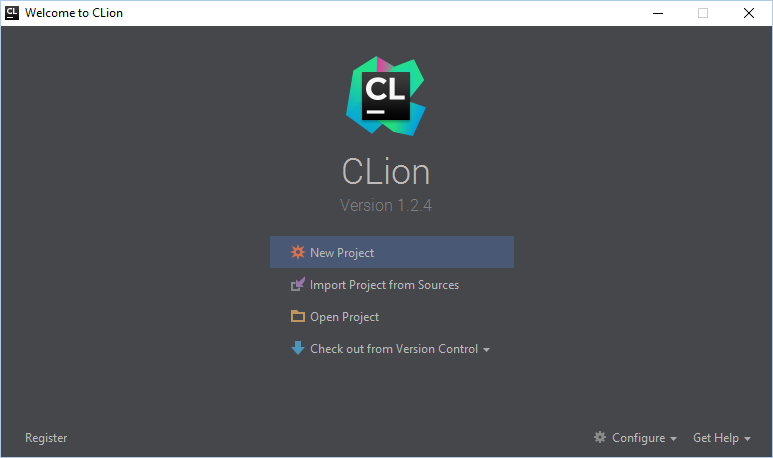
\includegraphics[width=\textwidth]{../Resources/lab0/image8.png}

\begin{enumerate}
\def\labelenumi{\arabic{enumi}.}
\setcounter{enumi}{1}
\item
  Wait until symbols are loaded
\item
  Create a \emph{*.cpp} file
\end{enumerate}

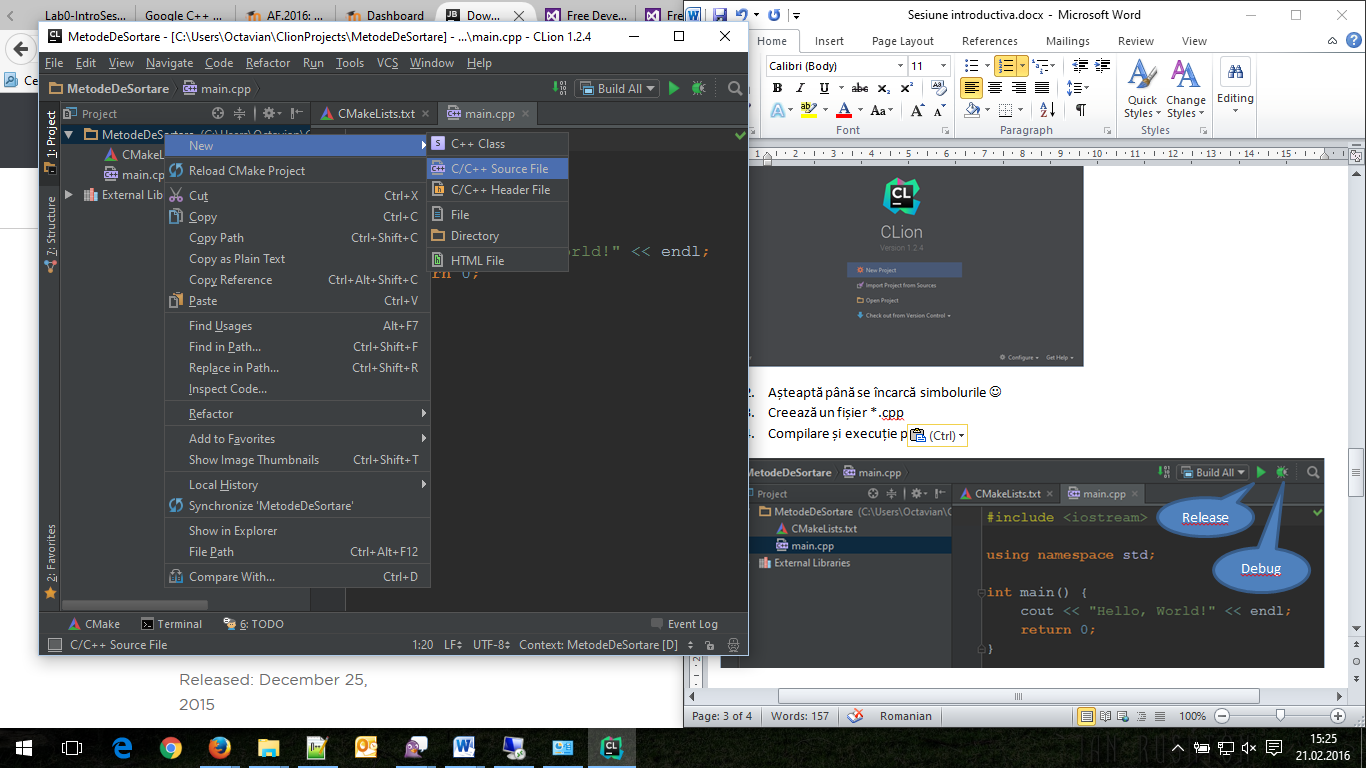
\includegraphics[width=\textwidth]{../Resources/lab0/image9.png}

\begin{enumerate}
\def\labelenumi{\arabic{enumi}.}
\setcounter{enumi}{3}
\item
  Compile and execute program
\end{enumerate}

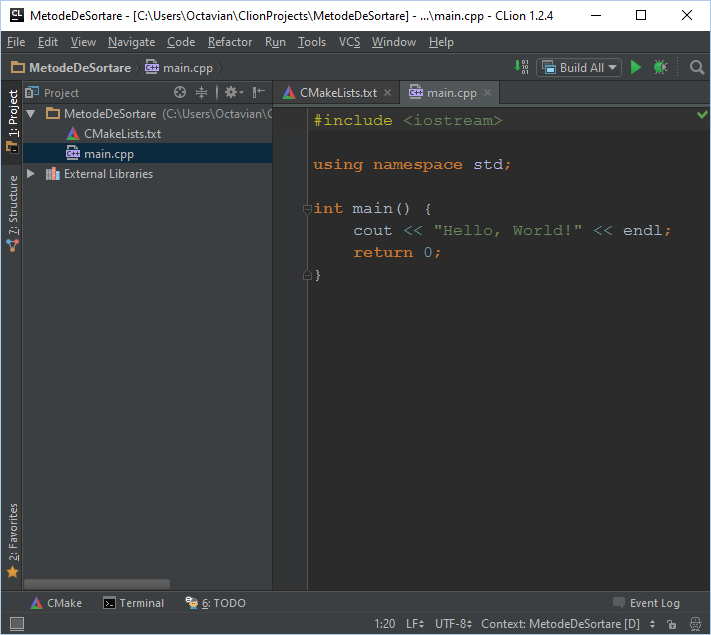
\includegraphics[width=\textwidth]{../Resources/lab0/image10.png}


\subsection{C/C++}\label{cc}

\subsubsection{Reading/writing files}\label{readingwriting-files}

\textbf{Exercise} - steps:

\begin{itemize}
\item
  Declare an array \emph{v} of length \emph{MAX\_SIZE} (a constant
  defined by you)
\item
  Read an \emph{n} from the keyboard
\item
  Open the \emph{input.txt} file, read \emph{n} numbers from it and save
  them in array \emph{v}
\item
  Save the \emph{n} numbers in the \emph{output.txt} file in
  \textbf{reverse} order
\end{itemize}

\subsubsection{Generating test cases}\label{generare-cazuri-de-testare}

To test the algorithms you will implement, you will need to use a series
of input data: sorted ascending arrays, sorted descending arrays, random
arrays, etc. Generating ascending/descending arrays should be
straightforward. For generating random arrays, you can use the
following:

\begin{itemize}
\item
  \emph{Profiler} library from Moodle (or
  \url{https://github.com/cypryoprisa/utcn-fa-profiler})
\item
  \emph{rand}(), \emph{srand}() methods, read:

  \begin{itemize}
  \item
    \url{http://www.cplusplus.com/reference/cstdlib/rand/}
  \item
    \url{http://www.cplusplus.com/reference/cstdlib/srand/}
  \item
    \url{http://www.cplusplus.com/reference/cstdlib/RAND_MAX/}
  \end{itemize}
\end{itemize}

\textbf{Exercise} - steps:

\begin{itemize}
\item
  Read \emph{n}, \emph{min} and \emph{max} from the keyboard
\item
  Generate a random array of \emph{n} elements with values bounded
  within \emph{min} and \emph{max}
\item
  The array must be different for each execution of the program
\item
  Add the array to the \emph{output.txt} file
\end{itemize}

\subsubsection{Generating plots}\label{generare-grafice}

For the generation of the charts, you can use:

\begin{itemize}
\item
  \emph{Profiler} library from Moodle (or
  \url{https://github.com/cypryoprisa/utcn-fa-profiler})
\item
  Microsoft Office Excel
\end{itemize}

\subsubsection{Microsoft Office Excel}\label{microsoft-office-excel}

You will need to create a file with the \emph{.csv} (comma-separated
values) extension. The file should have a structure similar to the
following:\\

n,assignments\_f1,comparisons\_f1,assignments\_f2,comparisons\_f2

100,1146,1228,1168,1268

200,2634,2820,2678,2878

300,4360,4635,4442,4742

400,6172,6520,6212,6612

500,8042,8458,8090,8590
\\\\
Legend:

\begin{itemize}
\item
  \emph{n}= the size of the problem (ex: lungimea șirului de intrare)
\item
  assignments\_f1= the number of assignments for the best-case scenario
  of method 1
\item
  comparisons\_f2= the number of assignments for the best-case scenario
  of method 2
\end{itemize}

\textbf{Caution:} If you open the CSV file in Excel and the values
appear in a single column, it means you should use a different delimiter
character (e.g., use a semicolon ";").

After you\textquotesingle ve opened the CSV file in Excel, select all
the values and create a \emph{PivotChart}.

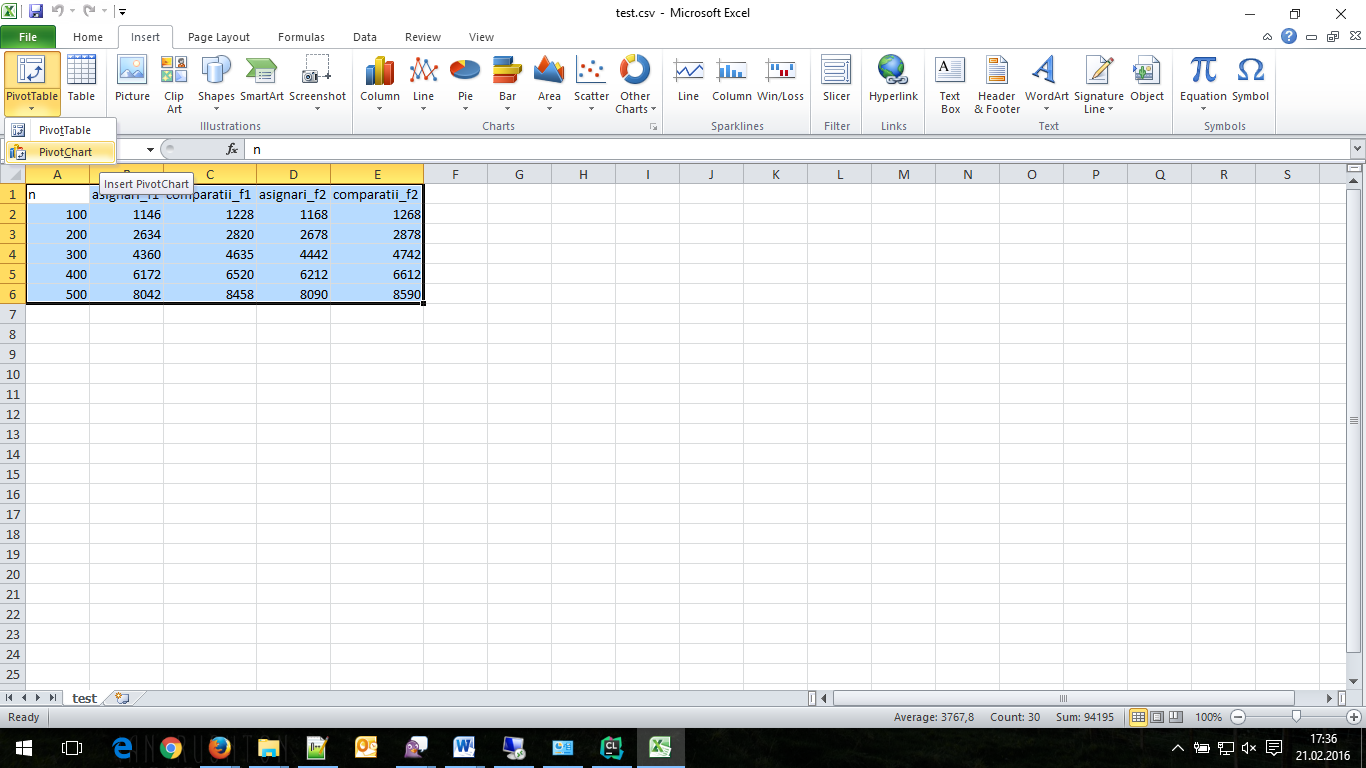
\includegraphics[width=\textwidth]{../Resources/lab0/image11.png}

After you click "\emph{Ok}," the window should look like the picture
below.

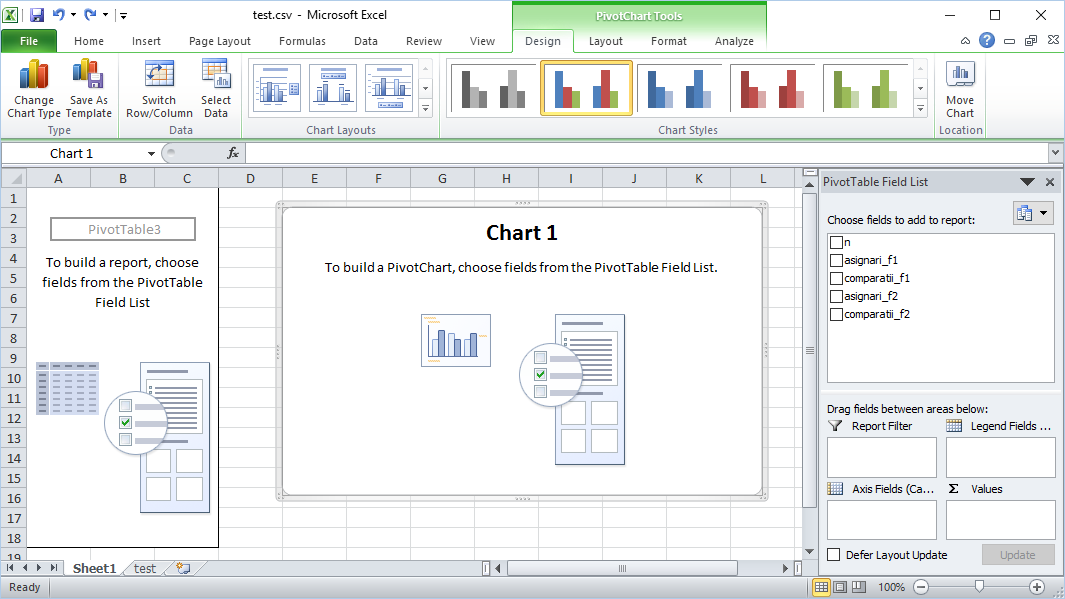
\includegraphics[width=\textwidth]{../Resources/lab0/image12.png}

In the left panel, drag "\emph{n}" to the "\emph{Axis Fields}" area and
the other columns to the "\emph{Values}" area.

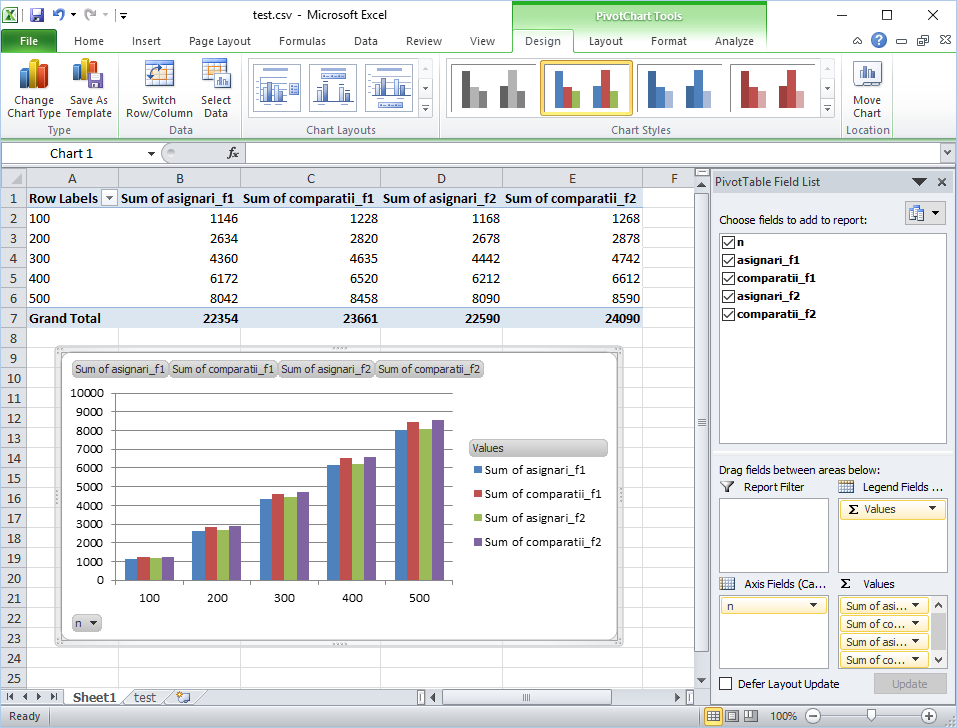
\includegraphics[width=\textwidth]{../Resources/lab0/image13.png}

Change the aggregation function from "\emph{Sum}" to "\emph{Average}":
Click on the black arrow in each row in the "\emph{Values}" area, then
choose "\emph{Value Field Settings}" and select "\emph{Average}." If
you\textquotesingle ve changed them correctly, the window should look
like the picture below.

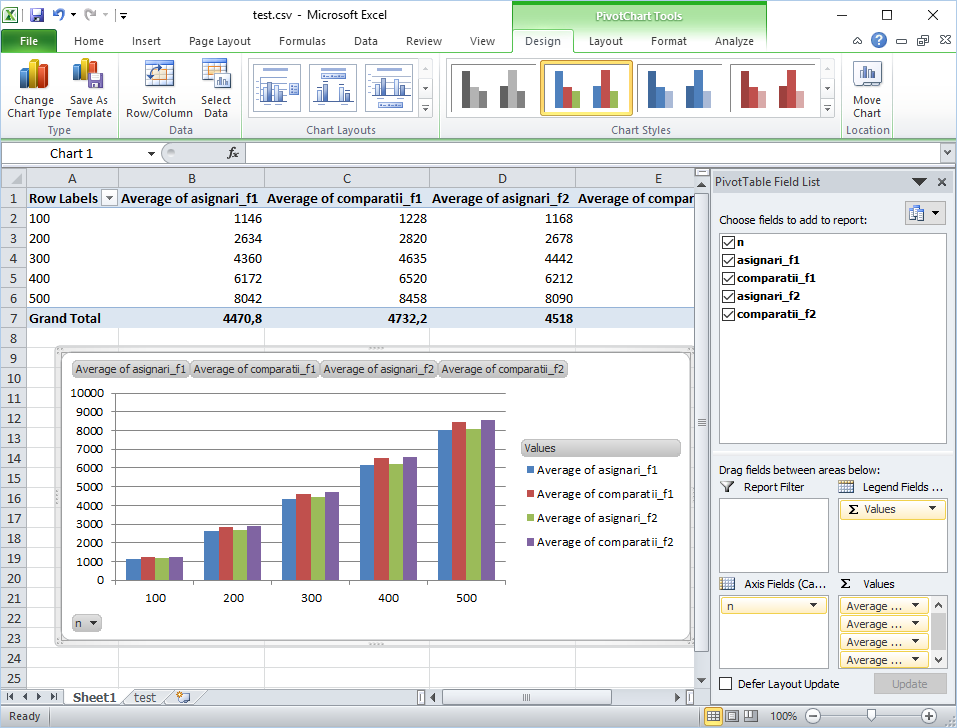
\includegraphics[width=\textwidth]{../Resources/lab0/image14.png}

The final step is to change the chart type to a line chart from
"\emph{Change Chart Type}." The final result should look like this:

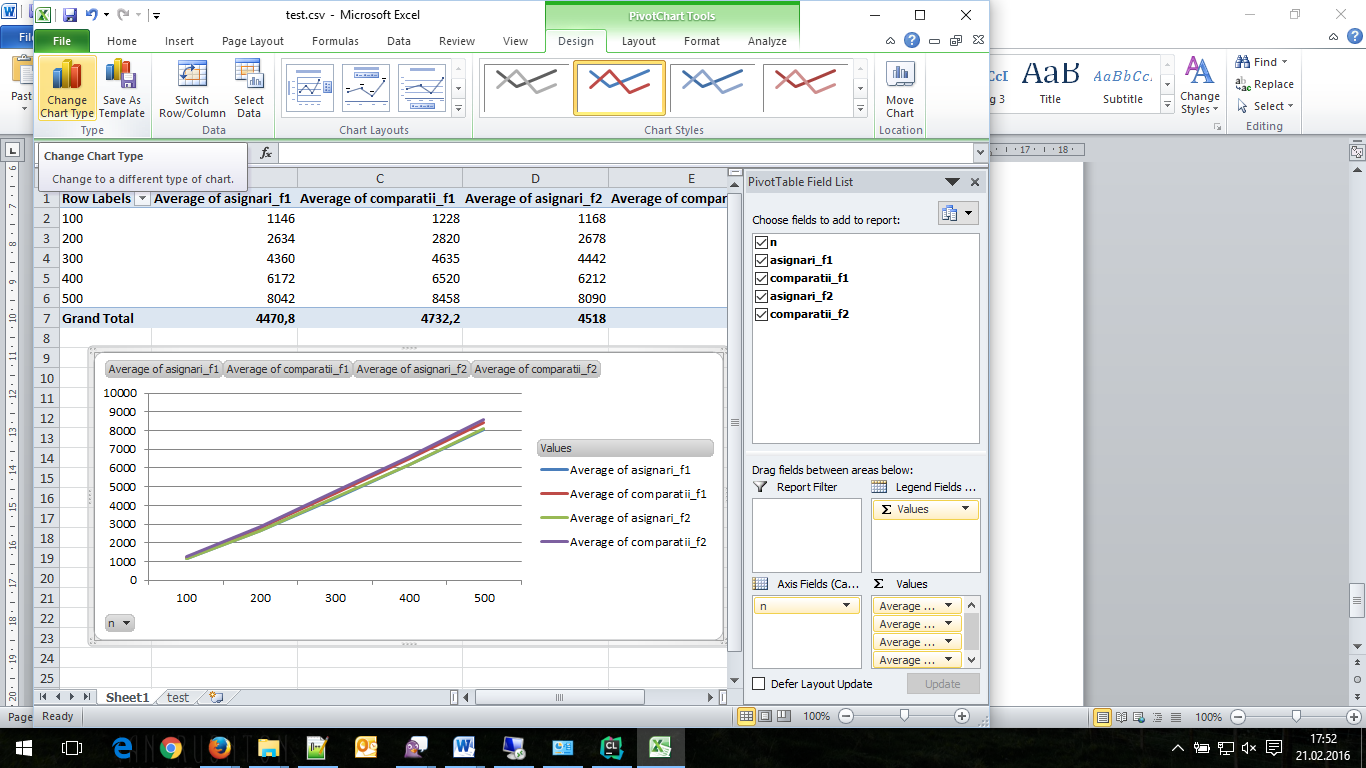
\includegraphics[width=\textwidth]{../Resources/lab0/image15.png}

\subsubsection{Exercise}\label{exerciux21biu}

Write a program that for each value \emph{n} of the interval \{100, 200,
\ldots, 10.000\} computes and adds into a file the following values:

n, 100*log(n), 10*n, n*log(n), 0.1*n\textsuperscript{2},
0.01*n\textsuperscript{3}

Use the values from the files to generate a chart depending on \emph{n}.

\end{document}